\documentclass[a4paper,12pt]{ctexart} 

% First, we usually want to set the margins of our document. For this we use the package geometry.
\usepackage[top = 2.5cm, bottom = 2.5cm, left = 2.5cm, right = 2.5cm]{geometry} 
\usepackage[T1]{fontenc}
\usepackage[utf8]{inputenc}

% The following two packages - multirow and booktabs - are needed to create nice looking tables.
\usepackage{multirow} % Multirow is for tables with multiple rows within one cell.
\usepackage{booktabs} % For even nicer tables.

% As we usually want to include some plots (.pdf files) we need a package for that.
\usepackage{graphicx} 

% The default setting of LaTeX is to indent new paragraphs. This is useful for articles. But not really nice for homework problem sets. The following command sets the indent to 0.
% \usepackage{setspace}
% \setlength{\parindent}{0in}

% Package to place figures where you want them.
\usepackage{float}

% The fancyhdr package let's us create nice headers.
\usepackage{fancyhdr}

\usepackage{amsmath,amsthm,mathabx}

% To make our document nice we want a header and number the pages in the footer.

\pagestyle{fancy} % With this command we can customize the header style.

\fancyhf{} % This makes sure we do not have other information in our header or footer.

\lhead{\footnotesize Probability and Statistics: Section 2.1}% \lhead puts text in the top left corner. \footnotesize sets our font to a smaller size.

%\rhead works just like \lhead (you can also use \chead)
\rhead{\footnotesize 吴梦轩} %<---- Fill in your lastnames.

% Similar commands work for the footer (\lfoot, \cfoot and \rfoot).
% We want to put our page number in the center.
\cfoot{\footnotesize \thepage} 

\begin{document}

\thispagestyle{empty} % This command disables the header on the first page. 

\begin{tabular}{p{15.5cm}}
{\large \bf Probability and Statistics} \\
Southern University of Science and Technology \\ 吴梦轩 \\ 12212006 \\
\hline
\\
\end{tabular}

\vspace*{0.3cm} %add some vertical space in between the line and our title.

\begin{center}
	{\Large \bf Section 2.1}
	\vspace{2mm}

	{\bf 吴梦轩}
		
\end{center}  

\vspace{0.4cm}

\subsection*{P46 Q1}

\begin{figure}[H]
	\begin{minipage}{0.5\textwidth}
		\centering
		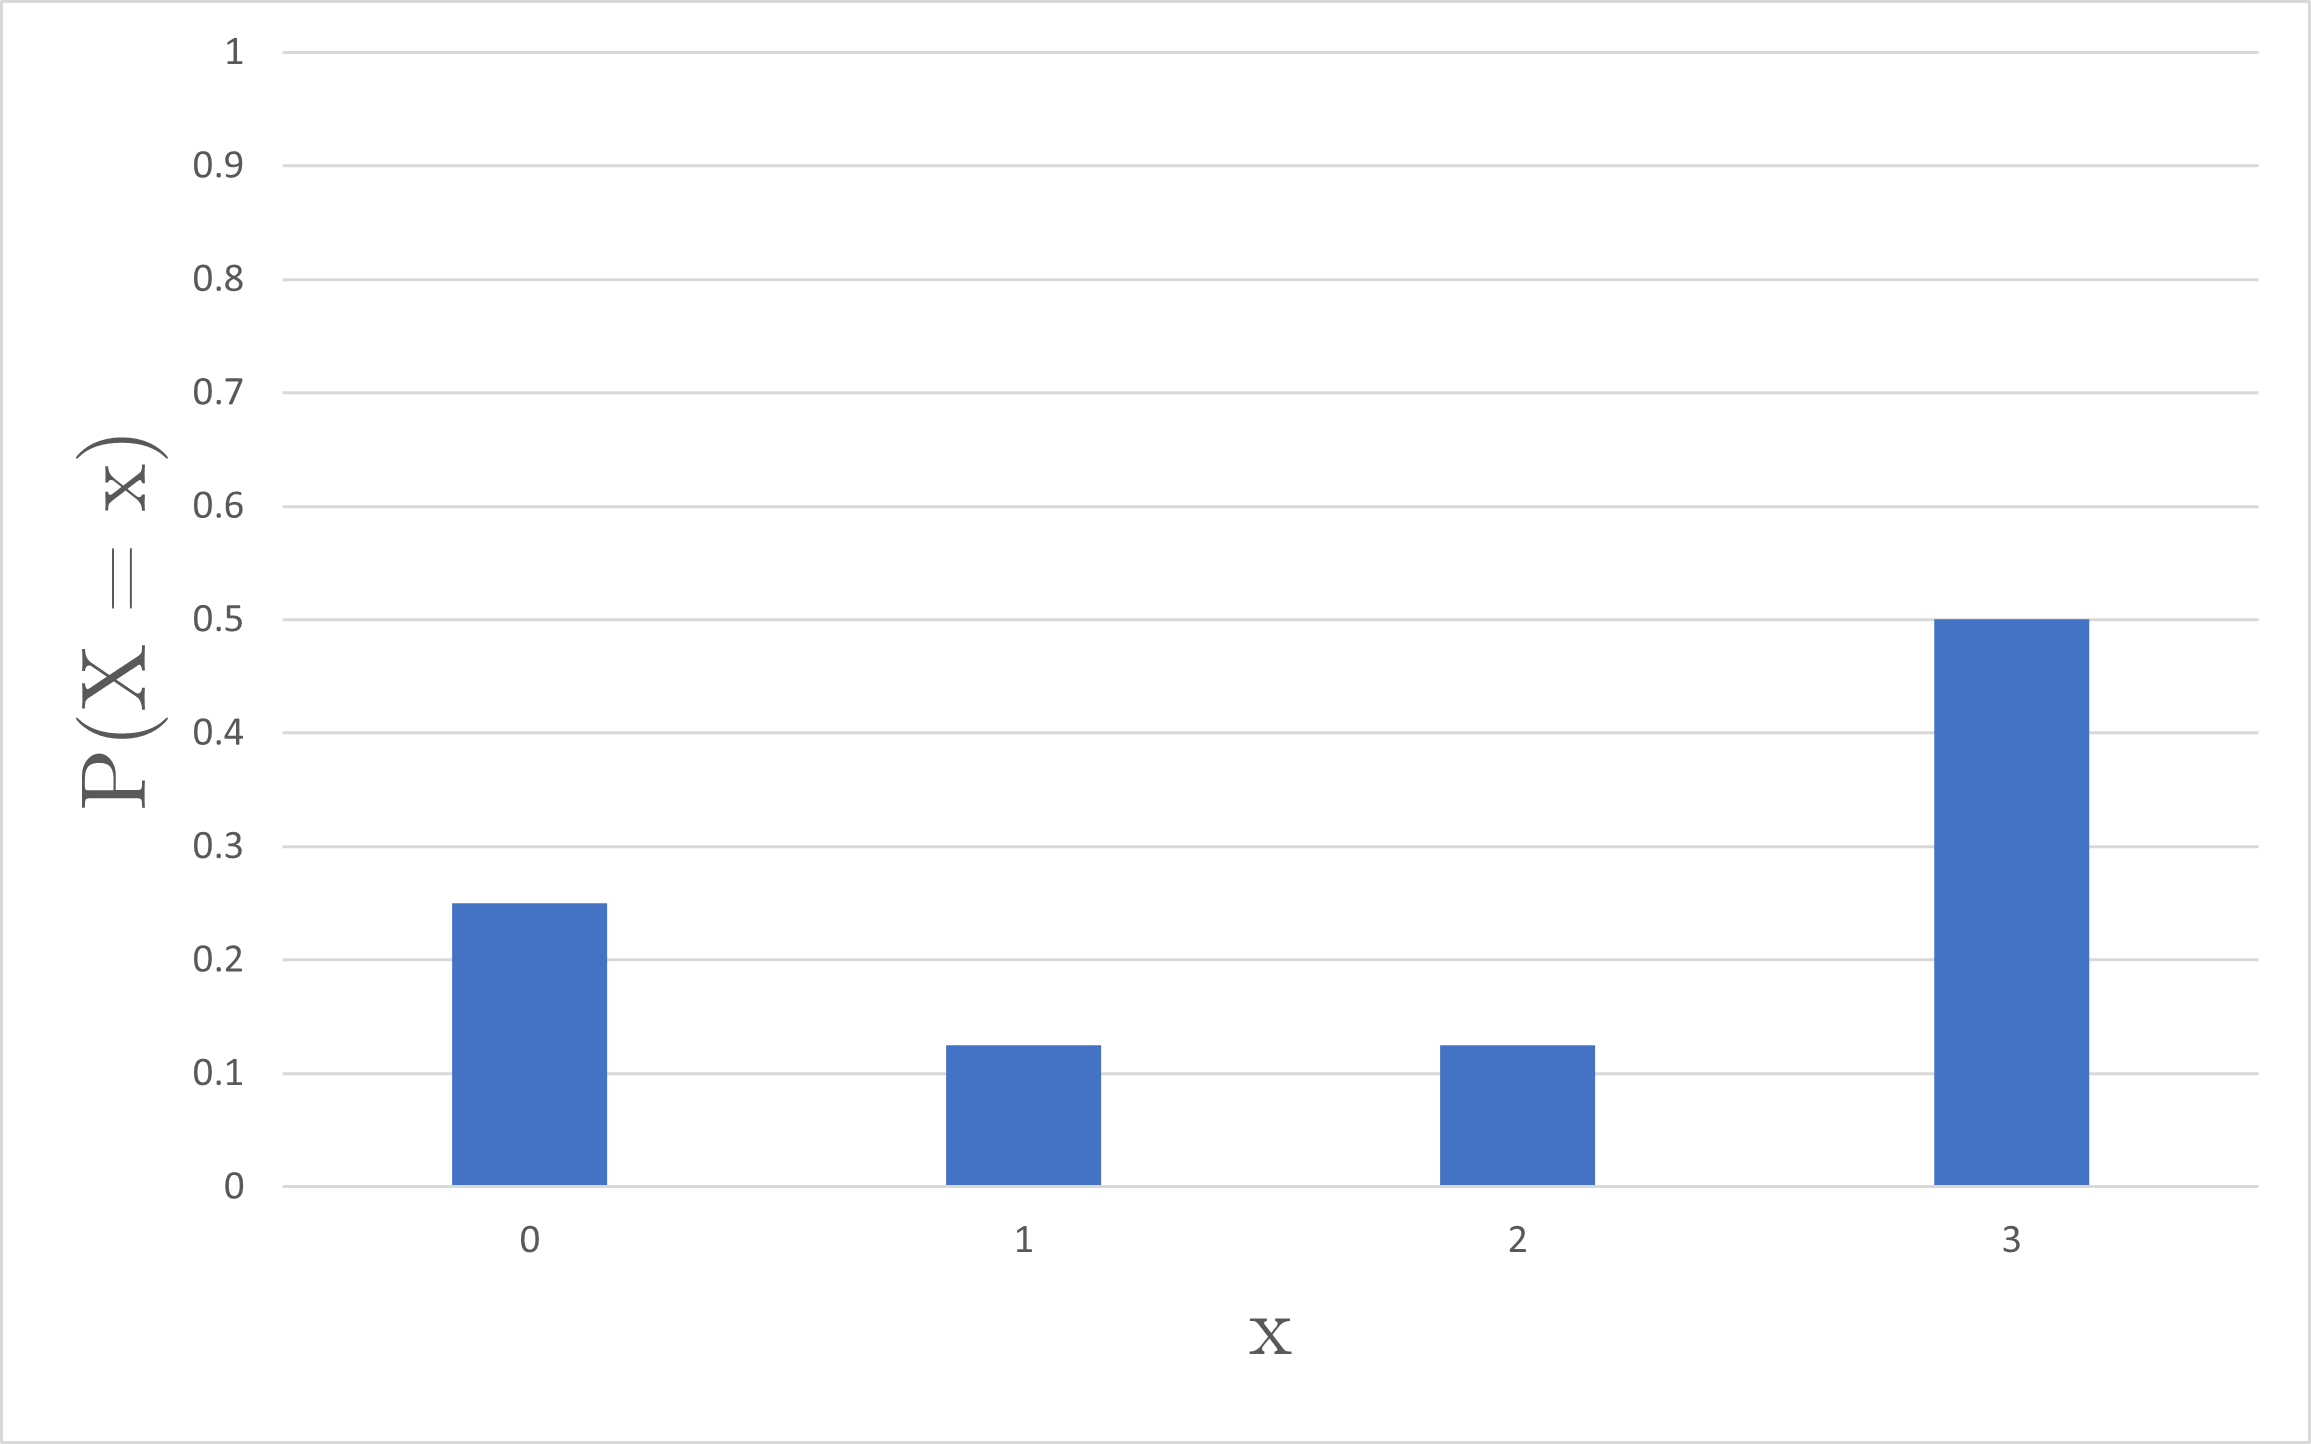
\includegraphics[width=\textwidth]{Figure1.png}
	\end{minipage}
	\begin{minipage}{0.5\textwidth}
		\centering
		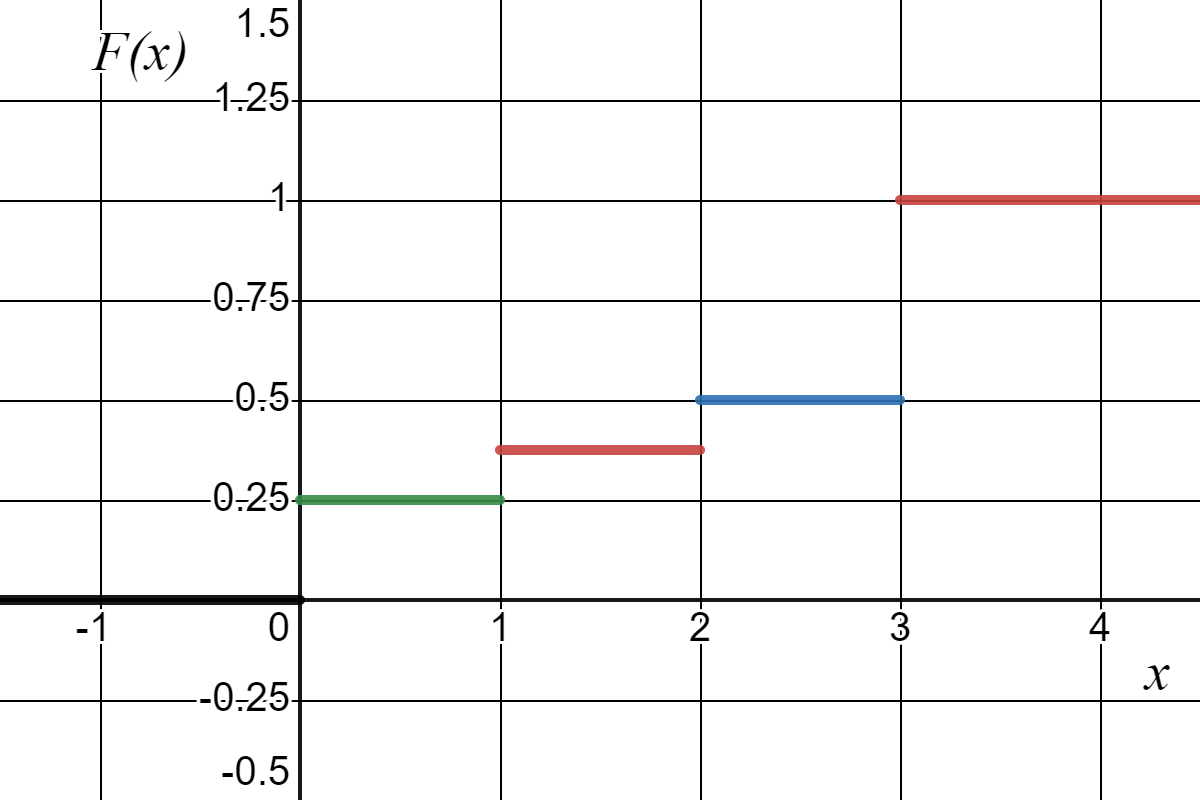
\includegraphics[width=\textwidth]{Figure2.png}
	\end{minipage}
\end{figure}

\subsection*{P46 Q15}
A队在5局比赛中至少获胜3次的概率为:
\begin{align*}
	P\{X \geq 3\} &= P\{X = 3\} + P\{X = 4\} + P\{X = 5\} \\
	&= C_2^2\ 0.4^3 \cdot 0.6^0 + C_3^2\ 0.4^3 \cdot 0.6^1 + C_4^2\ 0.4^3 \cdot 0.6^2 \\
	&= 0.064 + 0.1152 + 0.13824 \\
	&= 0.31744
\end{align*}

A队在7局比赛中至少获胜4次的概率为:
\begin{align*}
	P\{X \geq 4\} &= P\{X = 4\} + P\{X = 5\} + P\{X = 6\} + P\{X = 7\} \\
	&= C_3^3\ 0.4^4 \cdot 0.6^0 + C_4^3\ 0.4^4 \cdot 0.6^1 + C_5^3\ 0.4^4 \cdot 0.6^2 + C_6^3\ 0.4^4 \cdot 0.6^3 \\
	&= 0.0256 + 0.06144 + 0.09216 + 0.110592 \\
	&= 0.289792
\end{align*}

综上,5局3胜制对A队有利。

\subsection*{P47 Q31}

\subsubsection*{a.}

\begin{align*}
	P\{X \geq 1\} &= 1 - P\{X = 0\} \\
	&= 1 - \frac{(\lambda \cdot \frac{1}{6})^0}{0!} e^{-\lambda \cdot \frac{1}{6}} \\
	&= 1 - e^{-\lambda \cdot \frac{1}{6}}\\
	&= 1 - e^{-\frac{1}{3}}\\
	&\approx 0.28347
\end{align*}

\subsubsection*{b.}

\begin{align*}
	P\{X = 0\} &=\frac{(2t)^0}{0!} e^{-2t}\\
	&= e^{-2t}\\
	&\leq 0.5
\end{align*}

故$t \geq \frac{\ln 2}{2} \approx 0.34657$小时。

\subsection*{补充1}
\begin{align*}
	\sum_{x = 1}^{3} P\{X = x\} =& \sum_{x = 1}^{3} c(\frac{2}{3})^x\\
	=& c \cdot (\frac{2}{3} + \frac{4}{9} + \frac{8}{27})\\
	=& c \cdot \frac{38}{27}\\
	=& 1
\end{align*}

故$c = \frac{27}{38}$。

\subsection*{补充2}

已知
\begin{equation*}
	P\{X = k\} = \frac{\lambda^k}{k!} e^{-\lambda}
\end{equation*}

使第$k$项除以第$k-1$项,得
\begin{equation*}
	\frac{P\{X = k\}}{P\{X = k - 1\}} = \frac{\lambda^k}{k!} e^{-\lambda} \cdot \frac{(k - 1)!}{\lambda^{k - 1}} e^{\lambda} = \frac{\lambda}{k}\\
\end{equation*}

易知当$k \leq \lfloor \lambda \rfloor$时$\frac{\lambda}{k} \geq 1$,故$P\{X = k\}$在$k = \lfloor \lambda \rfloor$时取得最大值。

\subsection*{补充3}

\subsubsection*{(1)}

该随机变量服从超几何分布,故有:

\begin{align*}
	P\{X = 0\} =& \frac{C_{13}^3}{C_{15}^3}\\
	=& \frac{22}{35}
\end{align*}
\begin{align*}
	P\{X = 1\} =& \frac{C_{13}^2 \cdot C_2^1}{C_{15}^3}\\
	=& \frac{12}{35}
\end{align*}
\begin{align*}
	P\{X = 2\} =& \frac{C_{13}^1 \cdot C_2^2}{C_{15}^3}\\
	=& \frac{1}{35}
\end{align*}

综上:

\begin{center}
	\begin{tabular}{cccc}
		\toprule
		$X$ & 0 & 1 & 2 \\
		\midrule
		$P\{X = x\}$ & $\frac{22}{35}$ & $\frac{12}{35}$ & $\frac{1}{35}$ \\
		\bottomrule
	\end{tabular}
\end{center}

\subsubsection*{(2)}

\begin{figure}[H]
	\centering
	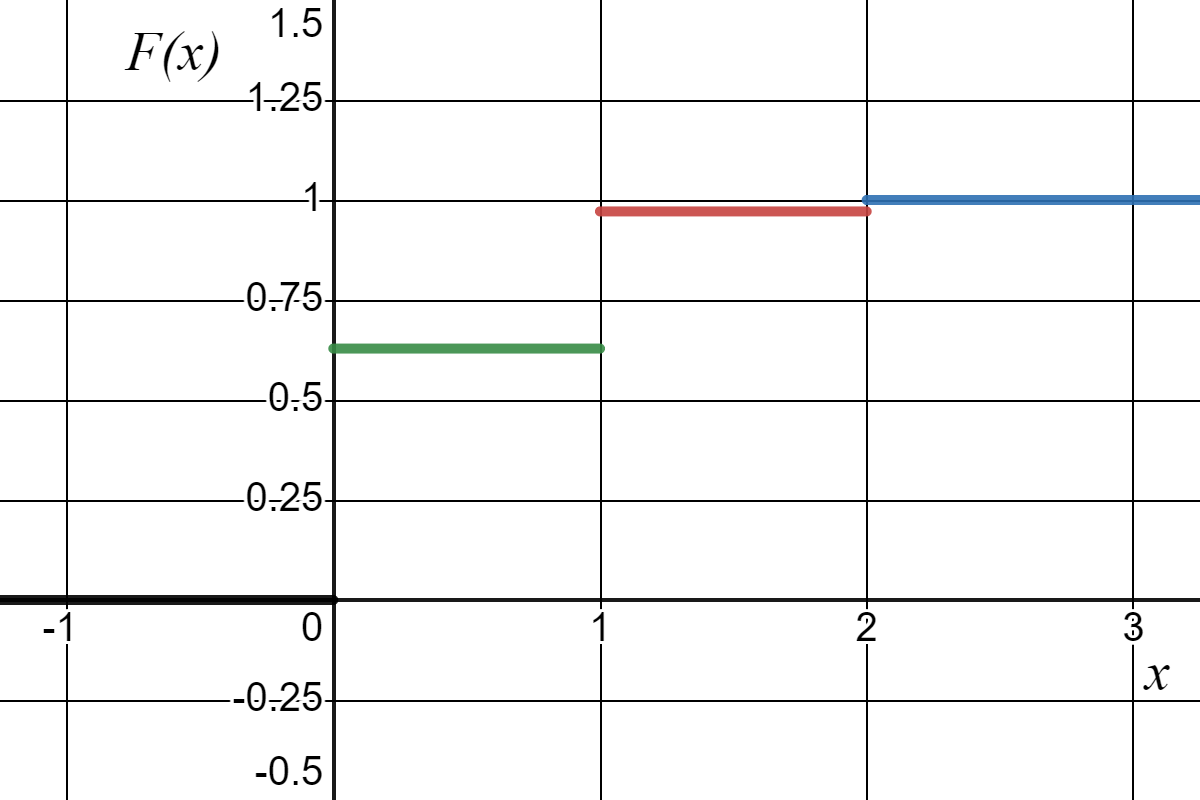
\includegraphics[width=0.5\textwidth]{Figure3.png}
\end{figure}

\subsubsection*{(3)}

\begin{equation*}
	P\{X \leq \frac{1}{2}\} = P\{X = 0\} = \frac{22}{35}
\end{equation*}
\begin{equation*}
	P\{1 < X \leq \frac{3}{2}\} = 0
\end{equation*}
\begin{equation*}
	P\{1 \leq X \leq \frac{3}{2}\} = P\{X = 1\} = \frac{12}{35}
\end{equation*}
\begin{equation*}
	P\{1 < X < 2\} = 0
\end{equation*}

\subsection*{补充4}

\subsubsection*{(1)}

记在一年中死亡的人数为$X$,该随机变量服从泊松分布。

若要使保险公司亏本,则有$2500 \cdot 12 < 2000 X$,即$X > 15$。
由泊松定理可知$\lambda = np = 2500 \times 0.002 = 5$。
则有:

\begin{align*}
	P\{X > 15\} =& 1 - P\{X \leq 15\}\\
	=& 1 - \sum_{x = 0}^{15} \frac{5^x}{x!} e^{-5}\\
	\approx& 1 - 0.99993\\
	=& 0.00007
\end{align*}

\subsubsection*{(2)}

解$2500 \cdot 12 - 2000X \geq 10000$,$2500 \cdot 12 - 2000X \geq 20000$,分别得到$X \leq 10$,$X \leq 5$。

\begin{align*}
	P\{X \leq 10\} =& \sum_{x = 0}^{10} \frac{5^x}{x!} e^{-5}\\
	\approx& 0.98630
\end{align*}
\begin{align*}
	P\{X \leq 5\} =& \sum_{x = 0}^{5} \frac{5^x}{x!} e^{-5}\\
	\approx& 0.61596
\end{align*}
\end{document}